\documentclass[11pt,letterpaper]{report}
\title{\Huge Parte-A}
\author{Work at Home Soft}
\usepackage[utf8]{inputenc}
\usepackage[spanish]{babel}
\usepackage{latexsym,amsmath,amssymb,amsthm}
\usepackage{graphicx}
\usepackage{pifont}
\usepackage[pdftex=true,colorlinks=true,plainpages=false]{hyperref}
\hypersetup{urlcolor=blue}
\hypersetup{linkcolor=black}
\hypersetup{citecolor=black}
\usepackage{lastpage}
\usepackage{url}
\usepackage{anysize}
\marginsize{3cm}{3cm}{1.2cm}{2.3cm}
\usepackage{fancyhdr}
\usepackage{anyfontsize}
\usepackage{tocbibind}
\usepackage{eso-pic}
\usepackage{mathptmx}
\usepackage{draftwatermark}
\usepackage{multirow}
\usepackage{pdfpages}
%\usepackage[usenames,dvipsnames]{xcolor}
%\usepackage{lipsum}
%-------------------------
\setlength{\parindent}{0in}
\pagestyle{fancy}
\lhead{}
\chead{{\Huge \tt Work at Home Soft S.R.L.}\\~\\~ }%\\{\tt \huge ~}\\{\tt \Large -~}}
\rhead{}
\lfoot{}
\cfoot{{\small \tt Av. Maria del Carmen Rodriguez s/n, Zona Pacata Baja Cochabamba.\\ Teléfono: +591-70797024}\\{\Large \tt \url{http://github.com/workathome}}}
\rfoot{\thepage/\pageref{LastPage}}
\renewcommand{\headrule}{{\color{black}\hrule width\headwidth height\headrulewidth \vskip-\headrulewidth}}
\renewcommand{\footrule}{{\color{black}%
\vskip-\footruleskip\vskip-\footrulewidth
\hrule width\headwidth height\footrulewidth\vskip\footruleskip}}
\renewcommand{\headrulewidth}{3pt}
\renewcommand{\footrulewidth}{3pt}
\footskip = 32pt
\headheight = 56pt
\headsep = 8pt
%--------------------------


\newcommand\BackgroundPic{
\put(50,707){
\parbox[b][\paperheight]{\paperwidth}{%
%\vfill
%\centering

\includegraphics[scale=0.83]{img/logo.png}%
%\vfill
}}}

%---------------------------
\SetWatermarkAngle{0}
\SetWatermarkLightness{0.1}
%\SetWatermarkFontSize{1cm}
\SetWatermarkScale{3}
\SetWatermarkText{
\includegraphics[scale=0.33]{img/marca_agua.png}}
%--------------------------------------

\begin{document}
%	\maketitle
\begin{titlepage}
	\begin{center}
		\vspace*{-1in}
		\begin{figure}[htb]
			\begin{center}
				
\includegraphics[width=8cm]{img/logo.png}
			\end{center}
		\end{figure}
		\Huge PARTE-A\\
		\vspace*{0.10in}
		\large CONVOCATORIA PÚBLICA\\
		\vspace*{0.10in}
		CPTIS-1707-2014\\
		\vspace*{0.1in}
		SISTEMA\\
		\vspace*{0.6in}
		\raggedright
		\begin{large}
			\textbf{CONSULTOR TIS:} Lic. Leticia Blanco Coca\\
			\textbf{RAZÓN SOCIAL DEL PROPONENTE :} Work at Home Soft \\
			\textbf{E-MAIL DEL PROPONENTE :} workathomesoft@gmail.com \\
			\textbf{REPRESENTANTE LEGAL DE LA EMPRESA :} Pe\~na Sahonero Erikc \\
			\textbf{TELÉFONO :} +591-70797024 \\
		\end{large}
	\end{center}
\end{titlepage}
\AddToShipoutPicture{\BackgroundPic}
%	\tableofcontents
~\\
~\\
\tableofcontents

\chapter{CONFORMACI\'ON DE LA GRUPO-EMPRESA}
\section{Raz\'on Social}
\begin{description}
\item {\bf Nombre de la empresa: } Work at Home Soft S.R.L.
\item {\bf Nombre Corto: } WHS S.R.L.
\item {\bf Tipo de Sociedad: } Sociedad de Responsabilidad Limitada
\item {\bf Logo: } 
\begin{center}

\includegraphics{img/logo.png}
\end{center}
\item {\bf Direcci\'on Legal: } Av. Maria del Carmen Rodriguez s/n, Zona Pacata Baja Cochabamba.
\item {\bf Representante Legal: } Erikc Pe\~na Sahonero 
\item {\bf Tel\'efono: } +591-70797024
\item {\bf E-mail: } workathomesoft@gmail.com
\item {\bf Socios: } 
\begin{itemize}
\item Cespedes Lopez Vladimir
\item Pe\~na Sahonero Erikc
\item Terrazas Mercado Michel
\item Zurita Ubaldino
\end{itemize}
\end{description}
\section{Misi\'on y Visi\'on }

\begin{description}
\item {\bf Misi\'on }\\
Work at Home Soft S.R.L., es una empresa que ofrece soluciones tecnol\'ogicas innovadoras en el campo de
desarrollo de software, garantizando soporte y actualizaciones constantes, adaptables a las
necesidades de nuestros clientes, fomentando su desarrollo y crecimiento, mediante un equipo de
profesionales en tecnolog\'ias de informaci\'on altamente competitivas.
\item {\bf Visi\'on }\\
Seguiremos construyendo nuestro futuro, siendo una empresa competitiva que ofrece productos de
software de excelente calidad y con altos niveles t\'ecnicos que satisfacen y sobrepasan las
necesidades de nuestros clientes, reconocida en Bolivia con presencia en el mercado.
\item {\bf Valores}
\begin{description}
\item [-]Trabajo en equipo:\\
Promoviendo y apoyando un equipo homog\'eneo e integrado.
\item [-]Colaboraci\'on:\\
Nos integramos con nuestros proveedores y clientes para mejorar d\'ia a d\'ia la calidad con los
mismos para satisfacer sus necesidades.
\item [-]Servicio\\
Cumplimos con nuestros compromisos y nos hacemos responsables de nuestro rendimiento
en todas nuestras decisiones y acciones, bas\'andonos en una gran voluntad de servicio por y
para nuestros clientes.
\item [-]Innovaci\'on y mejora continua\\
Nos damos cuenta de la importancia de mirar hacia el futuro, por tanto ofrecemos lo \'ultimo del
mercado para dar un apoyo y servicio \'optimo a nuestros clientes.
\item [-]Transparencia\\
La implicaci\'on y compromiso del personal no ser\'ia posible sin una absoluta transparencia en
los procesos, disponiendo el personal de la m\'axima información de la empresa.
\item [-]Comunicaci\'on\\
Promovemos y facilitamos la comunicaci\'on entre todos los niveles de la organizaci\'on,
disponiendo de herramientas eficaces, convocando los foros adecuados y con el compromiso
constante de la direcci\'on.
\item [-]Integridad y \'Etica\\
Promovemos un compromiso social y cumplimos nuestra normativa interna.
\item [-]Modelo de direcci\'on participativo\\
El personal de la empresa asume responsabilidades y participa en el proceso de toma de
decisiones.
\end{description}
\end{description}

\chapter{ SOLVENCIA T\'ECNICA }
\section{Equipo T\'ecnico}

\begin{center}
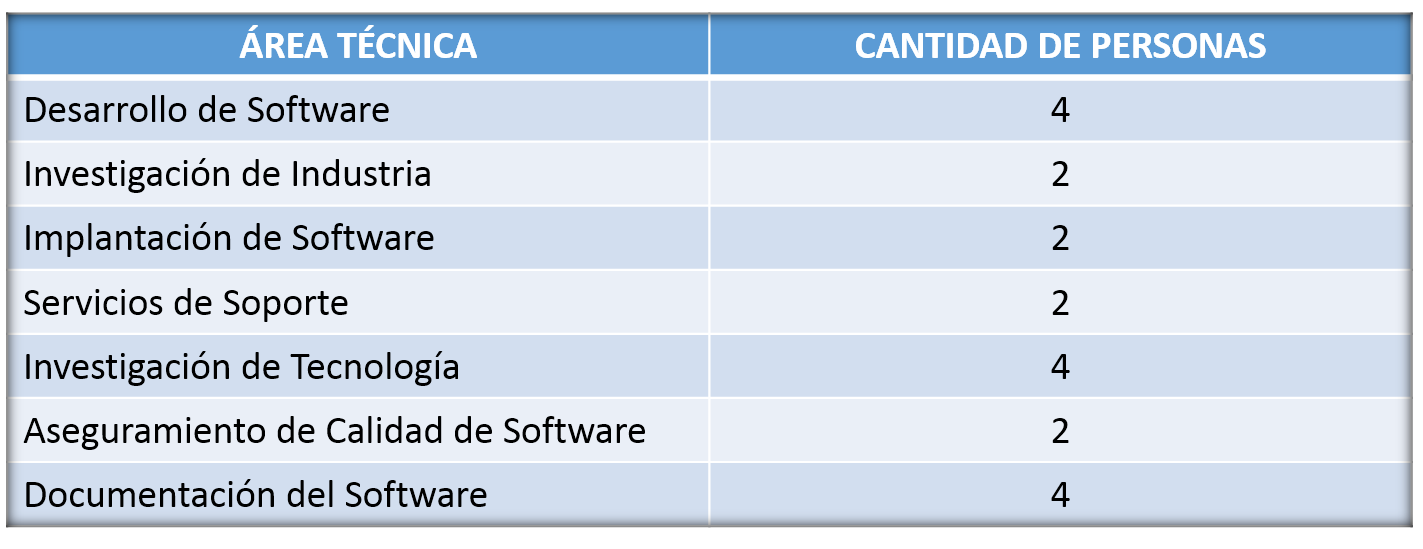
\includegraphics[scale=0.6]{img/tabla_personal.png}
\end{center}

%\begin{tabular}{|l|c|}
%\hline
% Área Técnica & Cantidad de Personas\\\hline
% Desarrollo de Software & 4\\\hline
% Investigación de Industria & 2\\\hline
% Implantación de Software & 4 \\\hline
% Servicios de Soporte & 1 \\\hline
% Investigación de Tecnología & 4\\\hline
% Aseguramiento de calidad de Software & 2\\\hline
% Documentación del Software & 4 \\\hline
%\end{tabular}\\
Tabla 2. Tabla del equipo técnico\\
La tabla 2 representa los componentes del equipo que darán soporte al proyecto en función del organigrama de la empresa. (Véase Figura 1.)

\begin{center}
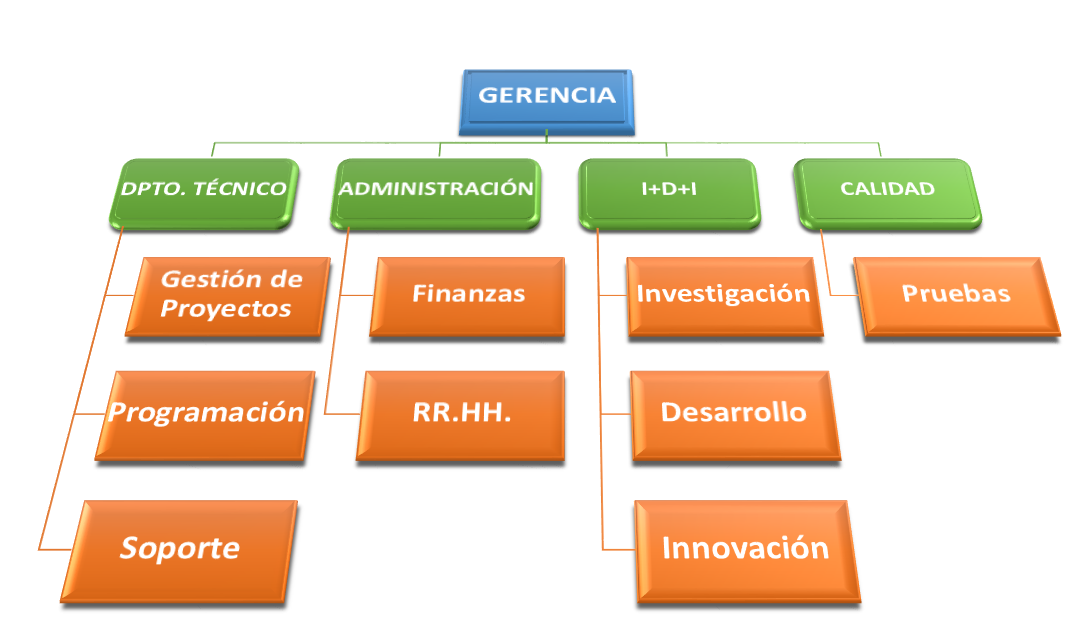
\includegraphics[scale=0.75]{img/diagrama_jerarquico.png}
\end{center}
\begin{center}
Figura 1: Organigrama de la grupo-empresa
\end{center}

\section{ Conocimiento Tecnol\'ogico }

\begin{itemize}
\item[-] Gestores de Base de Datos Relacionales
\begin{enumerate}
\item MySQL
\item PostgreSql
\end{enumerate}
\item[-] Gestores de Base de Datos No Relacionales
\begin{enumerate}
\item Mongodb
\item Cassandra
\end{enumerate}
\item[-] Lenguajes de Programación
\begin{enumerate}
\item Java
\item JavaFX
\item PHP
\item Python
\item Ruby
\item Haskell
\item Javascript
\item Lua
\item Visual Basic
\end{enumerate}
\item[-] Lenguaje de Marcado
\begin{enumerate}
\item CSS3
\item HTML5
\end{enumerate}
\item[-] Otras Herramientas
\begin{enumerate}
\item PowerDesigner
\item Navicat
\item Bluej
\item Sublime Text
\item \LaTeX
\item Eclipse
\item Netbeans
\item Rational Rose
\item Star UML
\item VMWare
\item Proteus
\item WireShark
\item Balsamiq
\end{enumerate}
\item[-] Plataformas y Frameworks
\begin{enumerate}
\item Nodejs
\item Laravel
\item CakePHP
\item Lungojs
\item Foundation css 
\end{enumerate}

\item[-] Sistemas Operativos
\begin{enumerate}
\item Windows
\item GNU/Linux
\end{enumerate}

\item[-] Experiencia Previa
\begin{enumerate}
\item Calculadora Básica, Científica, Estadística y de Bases (Taller de Programación)
\item Solitario Spyder (Taller de Programación)
\item Herramienta de gestión para la comercialización de productos en línea (Taller de Programación)
\item Automatización de registro de un hospital(Sistemas de Información II)
\item Venta de Matriculas mediante el sistema websiss (Sistemas de Información II)
\item Gestión de inmuebles dentro de una urbanización(Taller de Base de Datos)
\item Robot explorador "Picar" (Robótica)
\item Calculadora de Cálculos Estructurales (Calculo Numérico)
\item Control de venta de Lácteos (Data Warehouse)
\end{enumerate}
\end{itemize}
Para mayor información sírvase en revisar el Anexo 3.1, en el cual se encuentran los curriculum vitae de las integrantes del grupo empresa, los cuales avalan la formación, el conocimiento y la experiencia de las mismas.
\chapter*{ ANEXOS }
\section{ Curriculum de los Socios }
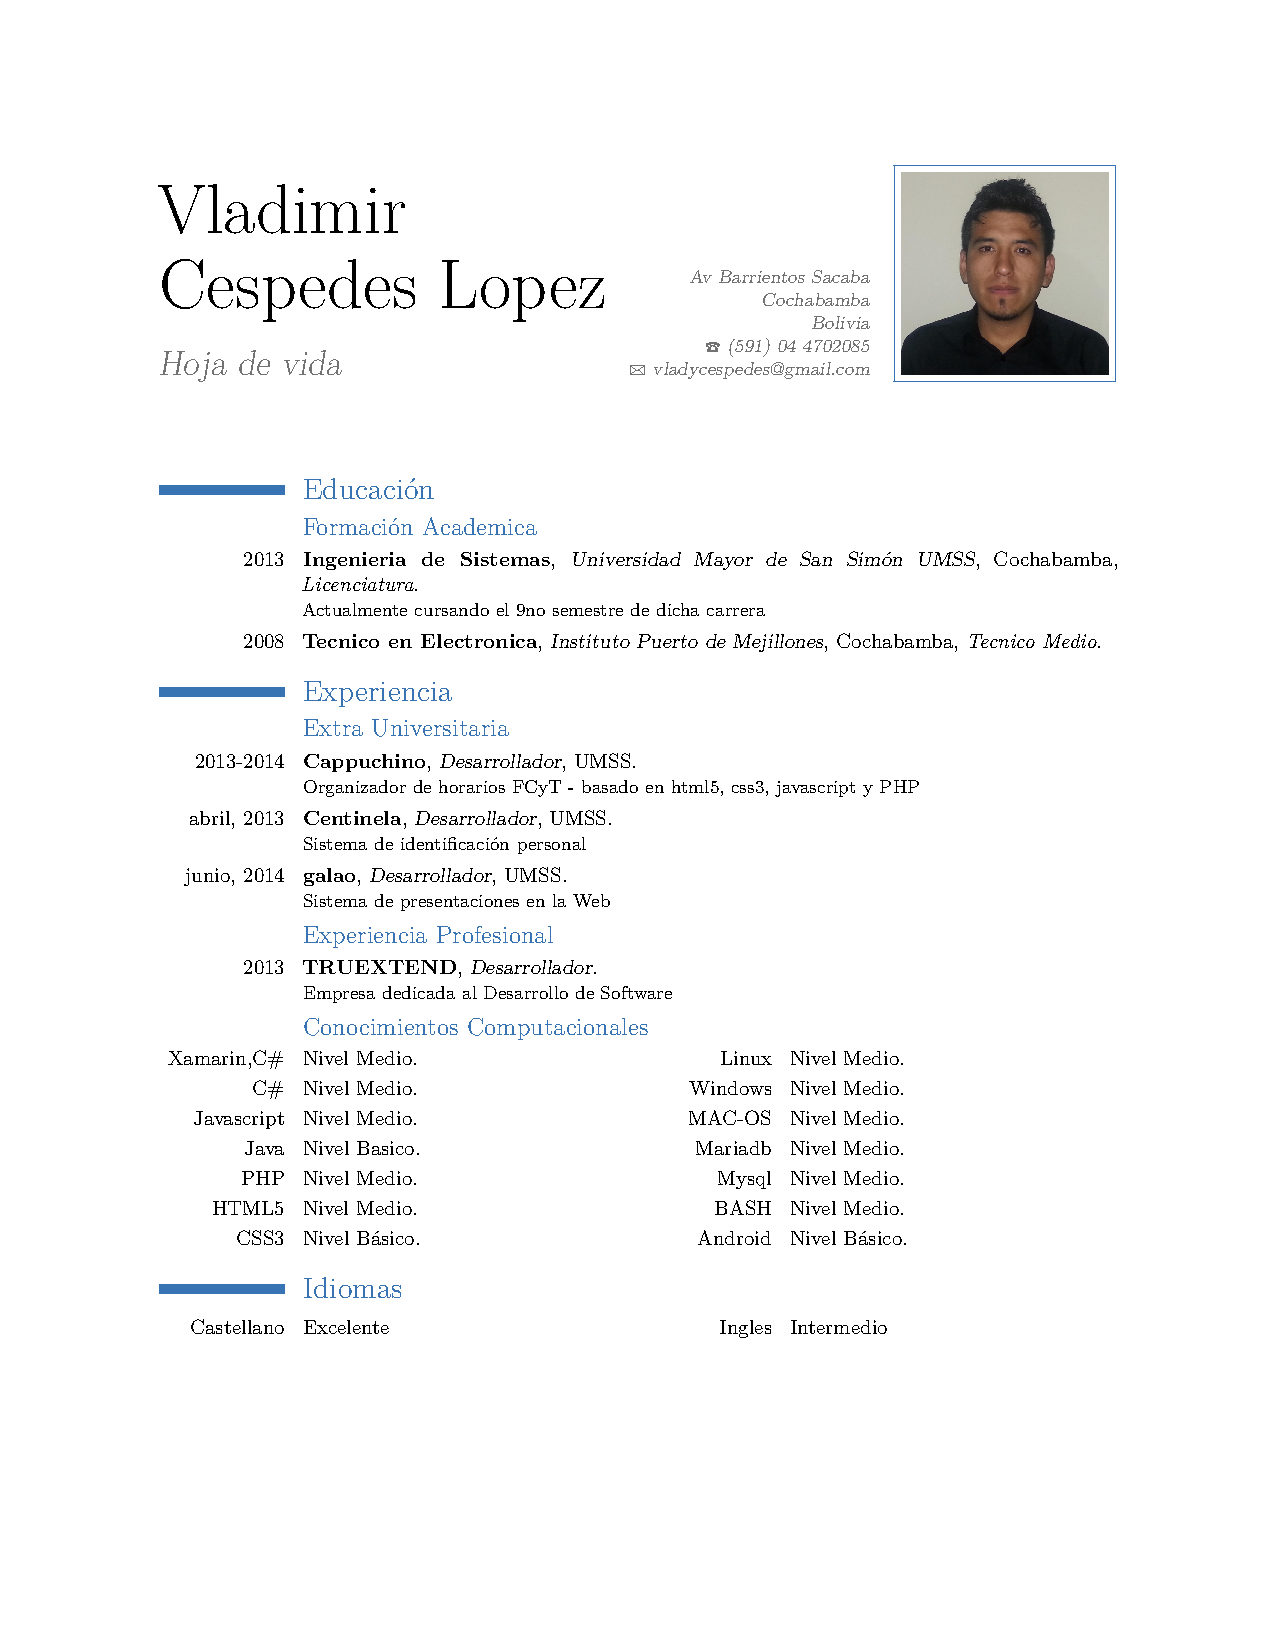
\includepdf[pages={1}]{../hojas_de_vida/vlady_cv.pdf}
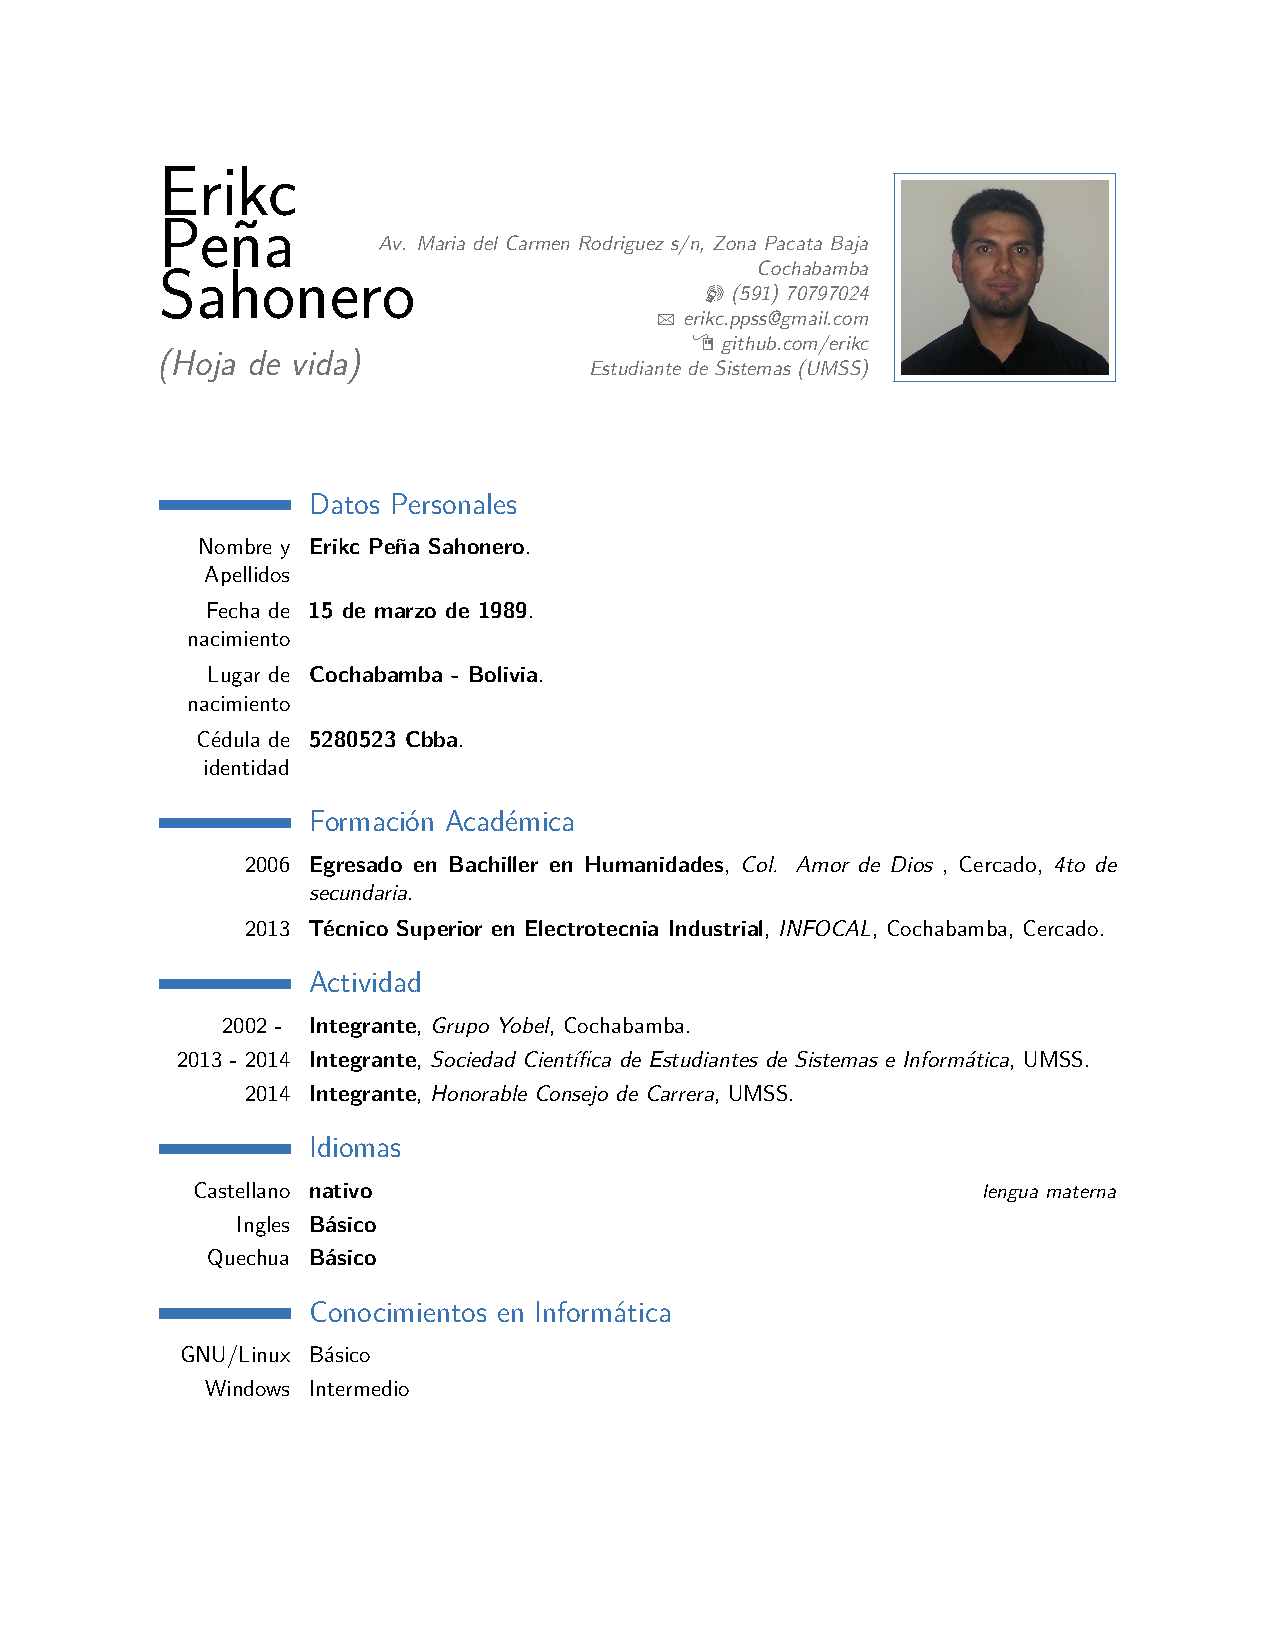
\includepdf[pages={1,2}]{../hojas_de_vida/erikc_cv.pdf}
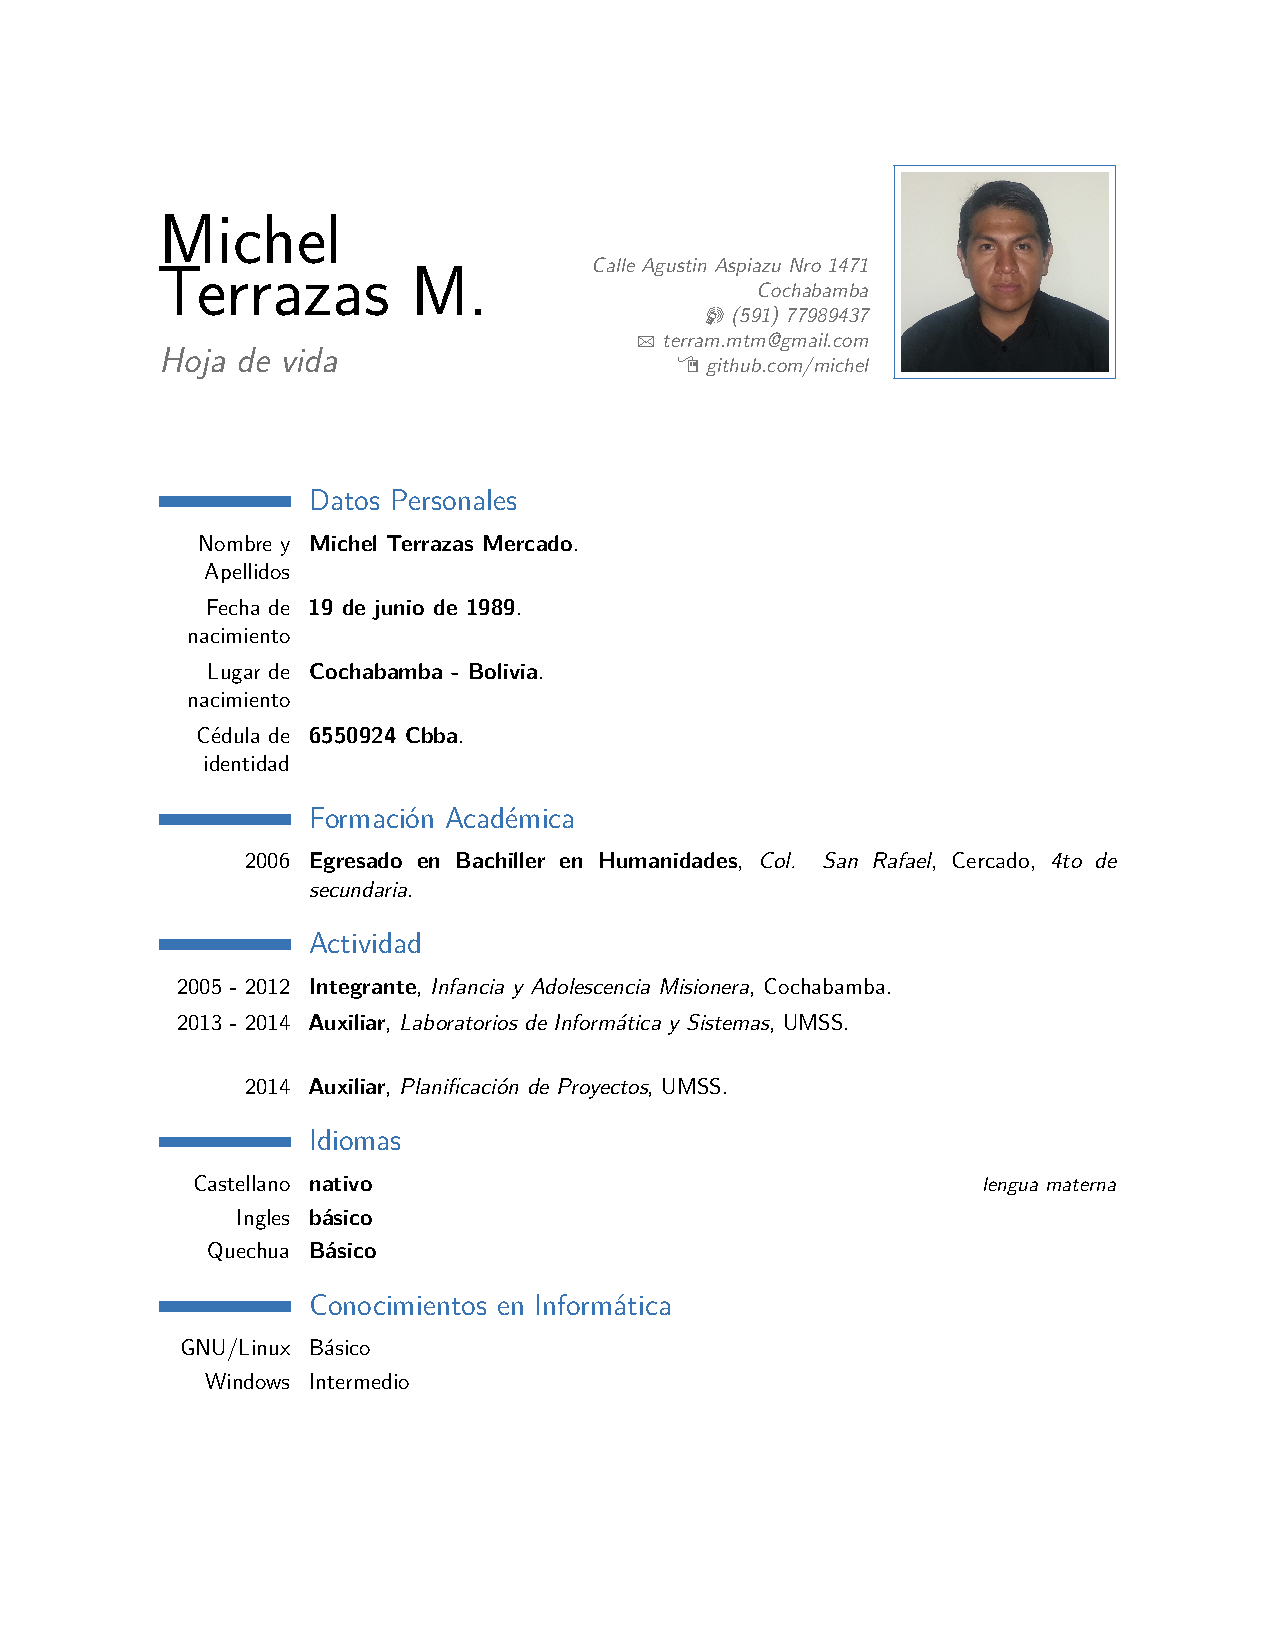
\includepdf[pages={1,2}]{../hojas_de_vida/michel_cv.pdf}
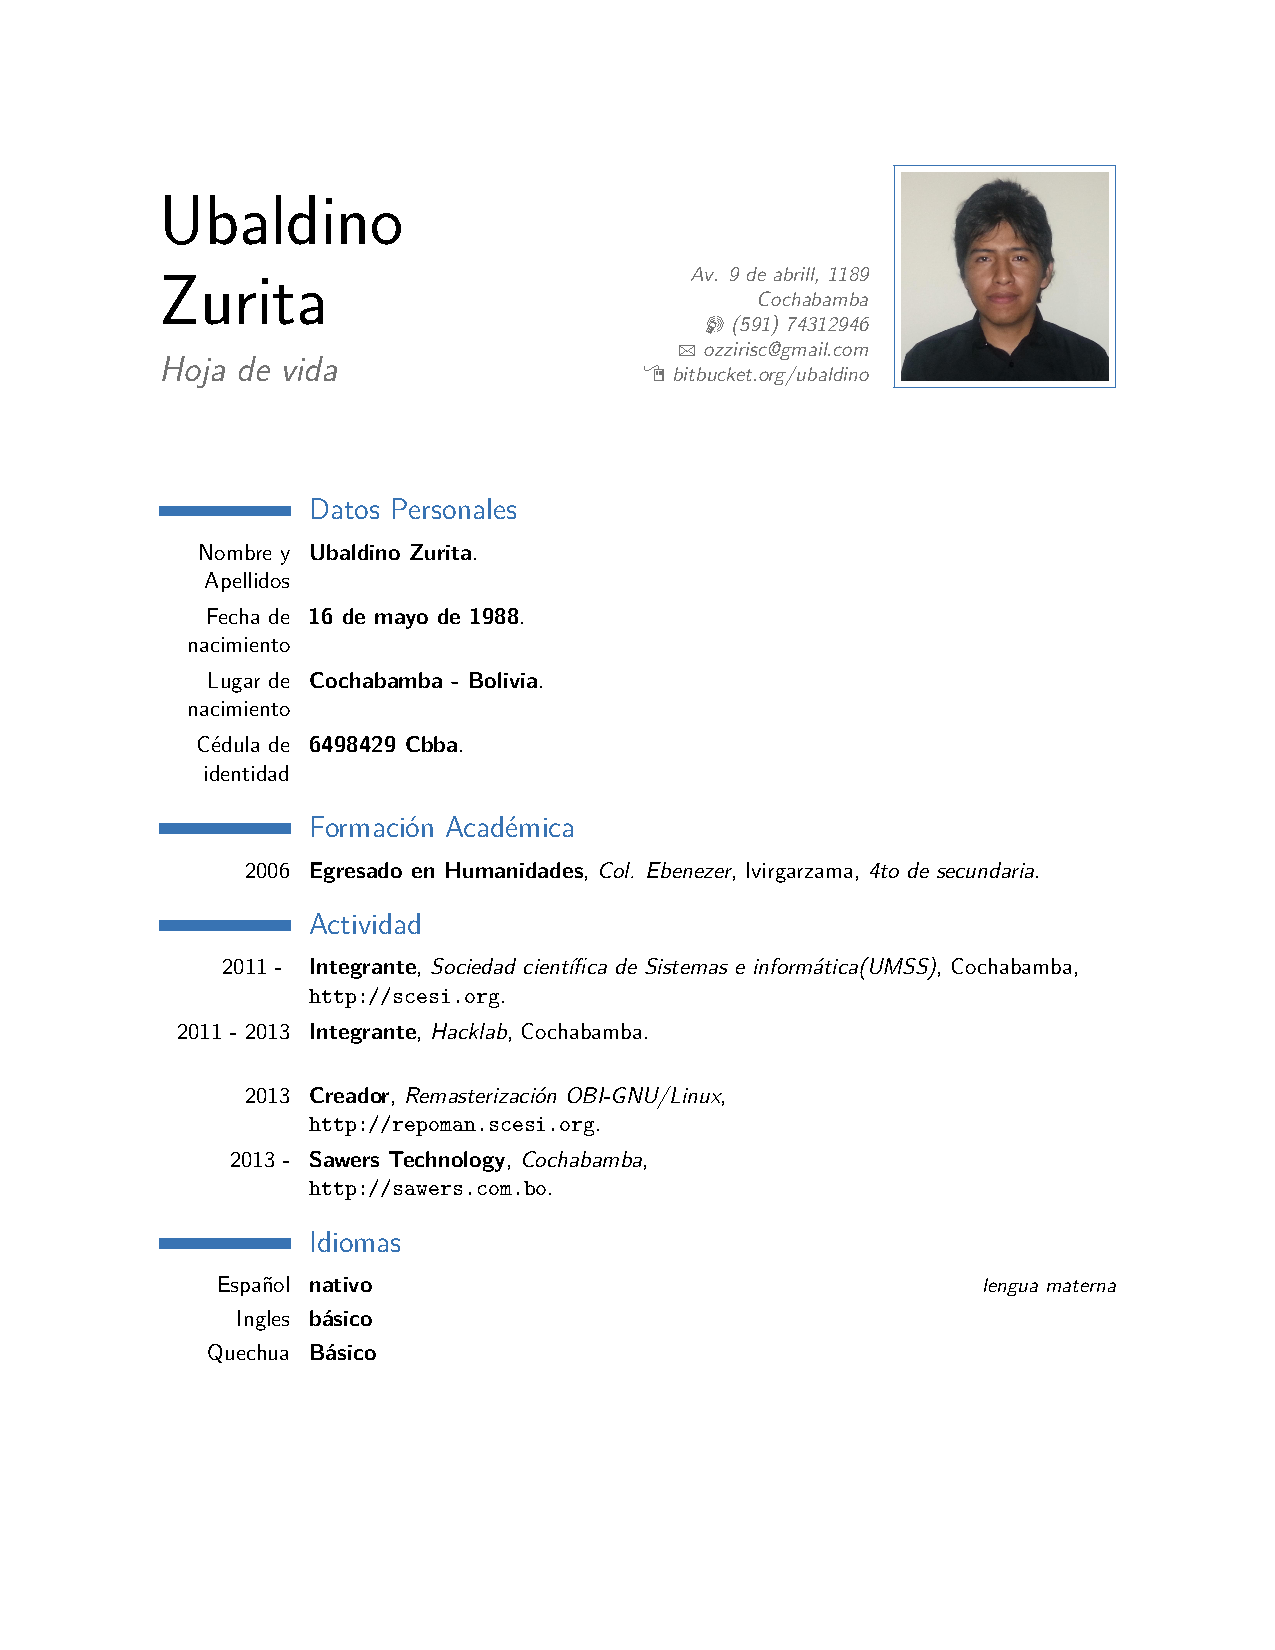
\includepdf[pages={1,2}]{../hojas_de_vida/ubaldino_cv.pdf}
\section{ Reglamento Interno }
\subsection{Capítulo I}
\begin{center}
{\bf Ámbito de aplicación}
\end{center}
\begin{enumerate}
\item Están sujetos al presente Reglamento, todas las personas que desempeñen cualquier trabajo a favor de la empresa Work at Home Soft S.R.L.
\item El presente Reglamento es de observancia obligatoria para los socios de la empresa.
\item Los socios de la empresa están obligados a cumplir también con las disposiciones de orden técnico y administrativo que dicte la misma, las cuales les serán dadas a conocer a través de los medios adecuados para el caso.
\end{enumerate}
\subsection{Capítulo II}
\begin{center}
{\bf Organización del personal}
\end{center}
\begin{enumerate}
\item La presidencia será rotativa, tendrá un periodo fijo de tiempo, que será definido en una asamblea.
\item Los trabajadores se consideran en:
\begin{description}
\item[Trabajadores permanentes:] aquellos cuya relación de trabajo tiene el carácter de tiempo indeterminado conforme al contrato individual o colectivo de trabajo.
\end{description}
\end{enumerate}
\subsection{Capítulo III}
\begin{center}
{\bf Lugar y tiempo de trabajo}
\end{center}
\begin{enumerate}
\item  Los trabajadores iniciarán y terminarán sus labores en los lugares que la empresa decide en consenso y deberán atender a cualquier otra actividad conexa a su ocupación principal.
\item  Al iniciarse la jornada de trabajo diariamente, los socios deberán registrar su ingreso en la herramienta de seguimiento.
\item En los días y horas que se establezcan para la limpieza del área de trabajo, instrumentos de trabajo o por cualquier otra causa, en los que el trabajador no se pueda dedicar a las labores que habitualmente desempeña, la empresa tiene el derecho de utilizar sus servicios y el trabajador el deber de prestarlos, en cualquier otra labor compatible que se le asigne, sin menoscabo de la retribución de su categoría. Al terminar esta circunstancia extraordinaria, el trabajador regresará a su puesto habitual.
\end{enumerate}
\subsection{Capítulo IV}
\begin{center}
{\bf Jornada de trabajo}
\end{center}
\begin{enumerate}
\item La jornada semanal de trabajo será de 20 horas tratándose del turno diurno. El horario u horarios que regirán en los distintos departamentos de la empresa será de lunes a viernes de las 14:00 a las 18:00, con una media hora para tomar alimentos.
\item El horario señalado podrá ser modificado a petición de la empresa y por necesidades de la misma, previo convenio con los socios.
\item Los trabajadores, sin excepción alguna, deberán estar en sus lugares de operación e iniciar sus labores exactamente a la hora señalada en el artículo 8; sin embargo, se contará con una tolerancia de 5 minutos, pasados los cuales se considerará como retardo al inicio de labores y posteriormente se procederá a tomar las medidas disciplinarias correspondientes.
\item Los trabajadores ejecutarán su trabajo con la intensidad, cuidado y esmero apropiados en los términos convenidos.
\end{enumerate}
\subsection{Capítulo V}
\begin{center}
{\bf Días de descanso y vacaciones}
\end{center}
\begin{enumerate}
\item La empresa concederá a sus trabajadores un día de descanso, por cada seis días de trabajo. Cuando no laboren durante los cinco días hábiles, la empresa cubrirá una sexta parte del salario, multiplicado por los días de la semana que se hubieren laborado.
\item La empresa concederá a sus trabajadores vacaciones anuales conforme al artículo 76 de la ley, en la inteligencia de que tales días serán pagados con salario íntegro.
\item Para el cómputo de las vacaciones del personal se incluirán únicamente los días laborables, entendiéndose como tales los que no estén incluidos en el descanso semanal.
\end{enumerate}

\subsection{Capítulo VI}
\begin{center}
{\bf Permisos}
\end{center}
Los trabajadores están obligados a solicitar los permisos para faltar a sus labores, por escrito dirigido a su jefe inmediato.
\begin{enumerate}
\item Toda falta no amparada con autorización escrita, se computará como injustificada.
\item Son consideradas faltas justificadas, sin el requisito del permiso autorizado por escrito, las que obedezcan a caso fortuito o fuerza mayor debidamente comprobada. La comprobación de la justificación deberá ser hecha por el trabajador dentro de la primera hora siguiente al inicio de la jornada a la cual no asistió.
\item El trabajador que necesite retirarse de la empresa durante la jornada de trabajo por enfermedad, razones personales o extraordinarias, deberá solicitar el permiso al jefe inmediato, quien le entregará la autorización correspondiente por escrito.
\end{enumerate}
\subsection{Capítulo VII}
\begin{center}
{\bf Lugar y días de pago}
\end{center}

\begin{enumerate}
\item Los salarios de los trabajadores serán cubiertos en el lugar donde se presten los servicios, y dentro de las horas de trabajo.
\item Si por ausencia del trabajador hubiere necesidad de que otra persona cobre su salario, ésta deberá presentar carta poder otorgada por el trabajador ausente y suscrita por dos testigos.
\item Todos los trabajadores están obligados a firmar los recibos de pago, listas de raya o cualquier documento que exija la empresa como comprobante del pago de los salarios. La negativa del trabajador a otorgar la firma de dichos documentos, relevará a la empresa de entregar los salarios respectivos.
\item Para los efectos del pago de vacaciones, la empresa pagará a los trabajadores los salarios correspondientes al período respectivo, el día anterior al inicio de su disfrute.
\item Durante el transcurso del proyecto se procurara designar las responsabilidades de forma equitativa a todos los miembros del equipo para que el salario sea el mismo hasta finalizar el proyecto.
\end{enumerate}

\subsection{Capítulo VIII}

\begin{center}
{\bf Medidas de higiene y seguridad}
\end{center}
\begin{enumerate}
\item El personal se abstendrá de realizar todo acto que pueda poner en peligro su propia seguridad, la de sus compañeros o las de la negociación.
\item Por ningún motivo, los trabajadores durante los períodos de incapacidades temporales médicas, ni las trabajadoras durante las incapacidades pre y postnatales deberán presentarse en los centros de trabajo.
\item En cada uno de los departamentos existirá un botiquín de emergencia con todos los implementos y útiles necesarios para la atención de los trabajadores que, en caso de accidente o enfermedad, requieran de un auxilio inmediato.
\item Para evitar accidentes de trabajo, los trabajadores deberán observar las siguientes reglas:
\begin{itemize}
\item Seguirán con todo cuidado y esmero las instrucciones que dicte la empresa respecto a la ejecución de sus trabajos, previsión de riesgos y observancia de medidas de cualquier índole encaminadas a tal efecto.
\item Usarán en todo caso el equipo e instrumentos de protección personales que sean necesarios en el desempeño de su trabajo.
\end{itemize}
\end{enumerate}
\subsection{Capítulo IX}
\begin{center}
{\bf Medidas disciplinarias}
\end{center}
\begin{enumerate}
\item Son causas de rescisión del contrato de trabajo, las señaladas en la Ley General del Trabajo.
\item Todas las faltas que impliquen incumplimiento de este Reglamento, a la Ley General del Trabajo, o al contrato de trabajo, que no ameriten la rescisión del contrato, serán sancionadas por la empresa con suspensión de labores hasta por ocho días.
El Departamento de Administración en cada caso hará las investigaciones correspondientes, escuchando siempre al trabajador, y como regla general notificará las normas disciplinarias por escrito.
\item Sanciones por ausencias injustificadas en períodos de 30 días:
\begin{description}
\item[- Una ausencia:] suspensión por un día, sin goce de sueldo.
\item[- Dos ausencias:] suspensión por tres días, sin goce de sueldo.
\item[- Tres ausencias:] rescisión de contrato.
\end{description}
\item Retardos injustificados en un período de 30 días:
\begin{description}
\item[- Un retardo:] amonestación.
\item[- Dos retardos:] suspensión de un día, sin goce de sueldo.
\item[- Más de tres retardos:] suspensión por dos días, sin goce de sueldo.
\end{description}
\item El tiempo no laborado por retardos, se descontará del sueldo del trabajador.
\item Los roles de trabajo tales como Scrum master y team (desarrolladores y testeadores) serán rotatorios para cada sprint durante el desarrollo del proyecto.
\item Los trabajadores que abandonen injustificadamente su lugar de trabajo con anticipación a la hora de la salida, serán sancionados con una amonestación o hasta con un día de suspensión, sin goce de sueldo, dependiendo de las consecuencias de su abandono en las actividades, la que además podría dar como resultado una causal de rescisión, en caso de causar un grave daño al patrimonio de la empresa.
\item Cualquier otra infracción a las disposiciones del presente reglamento será sancionada con una amonestación o con un día de suspensión de actividades, bajo el descuento salarial correspondiente, según la gravedad de la infracción.
\item Al finalizar un informe y/o sprint cada integrante de la empresa será sometido a una evaluación individual por parte de los mismos miembros, la calificación se realizara sobre un porcentaje de 100.
\begin{center}
{\bf Transitorios}
\end{center}
\begin{description}
\item[Primero.] La Comisión Mixta para la elaboración del presente documento deberá depositar el presente documento en la Junta de Conciliación y Arbitraje, dentro de los 2 días siguientes a su firma.
\item[Segundo.] El presente Reglamento deberá ser distribuido a todos los trabajadores que actualmente laboren en la empresa.
\item[Tercero.] Su vigencia iniciará a partir del día siguiente en que sea depositado ante la Junta de Conciliación y Arbitraje.
\item[Cuarto.] Este Reglamento no podrá ser modificado sino de común acuerdo entre empresa y trabajadores, notificando los cambios a la Junta respectiva, así como a todos los trabajadores de la organización.
\end{description}
\end{enumerate}
\begin{flushright}
\today
\end{flushright}

\chapter{ADJUNTO}
\section{Acta de constituci\'on}
En la notaria No5 de la ciudad de Cochabamba, estando presente el notario de fe p\'ublica Sr Antonio Mamani Quispe, siendo las 14:00 Hrs., del d\'ia 29 de agosto, del a\~no 2014 , se reunieron los socios:\\
\begin{enumerate}
\item Cespedes Lopez Vladimir con cedula de identidad Nro. 7879011 expedido en
COCHABAMBA
\item Pe\~na Sahonero Erikc con cedula de identidad Nro. 5280523 expedido en
COCHABAMBA
\item Terrazas Mercado Michel con cedula de identidad Nro. 6550924 expedido en
COCHABAMBA
\item Zurita Ubaldino con cedula de identidad Nro. 6498429 expedido en
COCHABAMBA
\end{enumerate}
Con motivo de fundar la grupo empresa Work at Home Soft S.R.L. ubicada en la Av. Maria del Carmen Rodriguez s/n, Zona Pacata Baja Cochabamba.
\subsection{ Socios } 
La sociedad est\'a conformada por socios igualitarios. Entendi\'endose con esto que todos los socios
son propietarios de la empresa Work at Home Soft S.R.L. en partes iguales, aportando cada socio
cuotas iguales, para el capital de la empresa y cada socio es totalmente responsable de los actos de
la empresa en s\'i misma.\\
\begin{enumerate}
\item Cespedes Lopez Vladimir, mayor de edad, h\'abil por ley, de nacionalidad BOLIVIANA, estado civil SOLTERO, de profesi\'on ESTUDIANTE, domicilio en Av. Barrientos Sacaba, titular de cedula de identidad Nro. 7879011 expedido en COCHABAMBA
\item Pe\~na Sahonero Erikc, mayor de edad, h\'abil por ley, de nacionalidad BOLIVIANA, estado civil SOLTERO, de profesi\'on ESTUDIANTE, domicilio en  Av. Maria del Carmen Rodriguez s/n, Zona Pacata Baja, titular de cedula de identidad Nro. 5280523 expedido en COCHABAMBA
\item Terrazas Mercado Michel, mayor de edad, h\'abil por ley, de nacionalidad BOLIVIANA, estado civil SOLTERO, de profesi\'on ESTUDIANTE, domicilio en Calle Agustin Aspiazu Nro 1471, titular de cedula de identidad Nro. 6550924 expedido en COCHABAMBA
\item Zurita Ubaldino, mayor de edad, h\'abil por ley, de nacionalidad BOLIVIANA, estado civil SOLTERO, de profesi\'on ESTUDIANTE, domicilio en Av. Dario Monta\~no Nro 9067, titular de cedula de identidad Nro. 6498429 expedido en COCHABAMBA
\end{enumerate}
Se ha resuelto en la fecha constituir una sociedad comercial de responsabilidad limitada que se desenvolver\'a de acuerdo a las disposiciones del c\'odigo de comercio y el presente contrato social.

\subsection{ Disposiciones generales }

\begin{description}
\item[ARTICULO 1$^{o}$.-] {\bf DENOMINACI\'ON.-}\\ La Sociedad de responsabilidad limitada, de nacionalidad boliviana, se denomina “Work at Home Soft”, S.R.L. Se regir\'a por lo dispuesto en estos estatutos, en su defecto por lo dispuesto en el Cap\'itulo XII de la ley 2/1995, de 23 de marzo, y, en lo no previsto en el mismo, por las dem\'as disposiciones que sean de aplicaci\'on a las Sociedades de Responsabilidad Limitada.
\item[ARTICULO 2$^{o}$.-] {\bf DOMICILIO.-}\\ El domicilio legal se fija en la Av. Maria del Carmen Rodriguez s/n, Zona Pacata Baja Cochabamba.
El \'organo de administraci\'on, podr\'a crear, suprimir y trasladar sucursales, agencias o delegaciones en cualquier punto del territorio boliviano o del extranjero, y variar la sede social dentro del mismo t\'ermino municipal de su domicilio.
\item[ARTICULO 3$^{o}$.-] {\bf OBJETO SOCIAL.- }
\begin{enumerate}
\item El objeto de la grupo-empresa es brindar a la sociedad cochabambina una nueva alternativa en cuanto a soluciones inform\'aticas orientada a empresas e instituciones, fomentando en todo momento las buenas relaciones con los clientes, buscando como primicia la satisfacci\'on de estos.
\item La consultor\'ia tecnol\'ogica y la ejecuci\'on de toda clase de proyectos tecnol\'ogicos. Formaci\'on, investigaci\'on y desarrollo en materia de tecnolog\'ia.
\end{enumerate}
\end{description}


\subsection{ Capital Social }
\begin{description}
\item[ARTICULO 4$^{o}$.-] {\bf CIFRA CAPITAL.-}\\ El capital social de la sociedad se fija en la cantidad de DOCIENTOS MIL BOLIVIANOS, dividido en cuatro cuotas, CINCUENTA MIL BOLIVIANOS por cada socio, y est\'a \'integramente desembolsado mediante aportaciones dinerarias de los socios. En la proporci\'on siguiente del cuadro de composici\'on.


\begin{tabular}{|c|c|c|c|c|c|}
\hline
Socio & {\tiny Aporte Equipo} & {\tiny Aporte Capital Efectivo } & {\tiny Puntos Capital Efectivo } & {\tiny Puntos Capital Esfuerzo } & {\tiny Total Puntos Capital} \\\hline
Vladimir Cespedes & 17500Bs & 32500Bs & 10000u & 10000u & 20000u \\\hline
Erikc Pe\~na & 17500Bs & 32500Bs & 10000u & 10000u & 20000u \\\hline
Michel Terrazas & 17500Bs & 32500Bs & 10000u & 10000u & 20000u \\\hline
Ubaldino Zurita & 17500Bs & 32500Bs & 10000u & 10000u & 20000u \\\hline
\end{tabular}

\item El capital de la empresa se medir\'a en puntos de capital. Donde un punto de capital equivale a:
\begin{enumerate}
\item CINCO 00/100 BOLIVIANOS( Bs 5 )
\item 80 horas/hombre trabajo al mes
\end{enumerate}



\end{description}
\subsection{ Duraci\'on }
\begin{description}
\item[ARTICULO 5$^{o}$.-] La sociedad se constituye por un tiempo indefinido, y dar\'a comienzo a sus operaciones sociales el d\'ia del otorgamiento de la escritura p\'ublica de constituci\'on.\\
En caso de {\bf disoluci\'on} se proceder\'a a la {\bf liquidaci\'on}.
\end{description}
\subsection{ Organizaci\'on de la Grupo-empresa }
\begin{itemize}
\item[a)] Niveles de organizaci\'on
\item[b)] \'Organos de la sociedad
\begin{enumerate}
\item Las asambleas de socios.
\item Las actas.
\item Presidencia
\end{enumerate}

\end{itemize}

\begin{itemize}
\item[a)] Niveles de la Organizaci\'on
\begin{description}
\item[Departamento T\'ecnico.-]
Este departamento se encarga de la gesti\'on de proyectos, del desarrollo e implantaci\'on de software, haciendo \'enfasis en la documentaci\'on y los servicios de
soporte respectivos.
\item[Departamento de Administraci\'on.-] Se encarga de las finanzas y administraci\'on en general de los recursos humanos de la empresa.
\item[Departamento de I+D+I.-] Esta \'area se encarga de la investigaci\'on, desarrollo e innovaci\'on tanto de la industria como de la tecnolog\'ia.
\item[Departamento de Calidad.-] Este departamento se dedica a dar cumplimiento a las pol\'iticas y procedimientos de gesti\'on de calidad.
\end{description}
\item[b)] \'Organos de la sociedad
\begin{description}
\item[1. ASAMBLEAS.-] La voluntad de los socios, expresada por mayor\'ia de votos, regir\'a la vida de la Sociedad con arreglo a la Ley.\\
Existen dos clases de asambleas las ordinarias y extraordinarias.\\
Las asambleas ordinarias se llevar\'ian a cabo UNA VEZ A AL MES A HORAS 14:00, con excepci\'on de algunas fiestas religiosas, durante al menos 2 a\~nos computables a partir de la fecha de inscripci\'on en el registro de comercio.\\
Las asambleas extraordinarias se llevaran a cabo cuantas veces se considere necesario.\\
Atribuciones de las asambleas:
\begin{enumerate}
\item Nombrar y remover al representante legal.
\item Aprobar los reglamentos de la sociedad.
\item Autorizar todo aumento o reducci\'on de capital social.
\item Modificar la escritura constitutiva.
\item Decidir acerca de la disoluci\'on y liquidaci\'on de la sociedad, retiro de socios, nombramiento y remoci\'on de liquidadores.
\item Cualquier otro tema de inter\'es de la sociedad, consignado en el orden del d\'ia.
\end{enumerate}
\item[2. ACTAS .-] Las actas estar\'an a cargo de un secretario de actas, designado en forma rotativa cuando as\'i lo dispongan los socios ya sea en asamblea ordinaria o extraordinaria, que ser\'a responsable de su existencia y de la exactitud de sus datos.\\
Se llevara un libro de actas donde constara un extracto de las deliberaciones y se consignaran las resoluciones adoptadas tanto en asamblea ordinaria y extraordinaria de Socios. Las actas ser\'an firmadas por todos los socios.

\item[3. PRESIDENCIA.-] Los socios del grupo-empresa Work at Home Soft S.R.L. designan al Sr. ERIKC PE\~NA SAHONERO como titular de dicha funci\'on por un periodo de tiempo determinado.

\item[ARTICULO 6$^{o}$.-] {\bf \'ORGANO DE ADMINISTRACI\'ON.-}\\  La gesti\'on y el ejercicio de la representaci\'on de la sociedad corresponder\'an a Administradores Mancomunados nombrados por la Junta General de Socios, debiendo ser un m\'inimo de dos Administradores y un m\'aximo de tres.\\
El \'Organo de Administraci\'on ejercer\'a su cargo por tiempo indefinido, salvo que la Junta general, con posterioridad a la constituci\'on, determine su nombramiento por plazo determinado.\\
El cargo de Administrador/a ser\'a gratuito.

\item[ARTICULO 7$^{o}$.-] {\bf FACULTADES DEL ADMINISTRADOR/A.-}\\ La representaci\'on de la Sociedad en juicio y fuera de \'el corresponder\'a a todos los Administradores Mancomunados nombrados en la forma prevista por la Ley y estos estatutos.\\
La representaci\'on se extender\'a a todos los actos comprendidos en el objeto social, incluidos aquellos que tengan car\'acter complementario o accesorio.\\
A efectos meramente enunciativos, se hace constar que los Administradores podr\'an realizar, entre otros, los siguientes actos y negocios jur\'idicos que se especificar\'a en la secci\'on de {\it R\'egimen disciplinario}.

\end{description}

\end{itemize}

\subsection{ R\'egimen disciplinario (derechos y obligaciones de los socios) }
\begin{description}
\item[ARTICULO 8$^{o}$.-] Los socios tendr\'an los siguientes derechos:\\ 
\begin{enumerate}
\item Voz y voto en las asambleas generales bien sean \'estas ordinarias o extraordinarias, en los t\'erminos y condiciones previstos en los presentes Estatutos.
\item Elegir y ser electos para ocupar cargos en el Consejo Directivo o en el Comit\'e de Vigilancia.
\item Percibir sus regal\'ias y obtener la documentaci\'on que sustente las respectivas liquidaciones.
\item Solicitar informes respecto al estado financiero de la Sociedad y, en general, sobre la marcha de todos los asuntos que les incumban.
\item Solicitar y obtener informes desglosados de las cantidades que les correspondan en concepto de regal\'ias que sus obras hayan generado.
\item Acceder a los beneficios de seguridad social que otorgue cada rama en los t\'erminos que establezcan los reglamentos respectivos.
\item Impugnar judicialmente las resoluciones de la Asamblea cuando sean contrarias a la Ley o a los presentes Estatutos. El derecho de impugnaci\'on deber\'a hacerse valer ante autoridad competente en un t\'ermino de treinta d\'ias de calendario contados a partir del d\'ia siguiente en que se haya celebrado la Asamblea.
\item Denunciar ante el Comit\'e de Vigilancia o ante el Instituto Nacional del Derecho de Autor los actos realizados por los \'Organos de Gobierno de la Sociedad que considere contrarios a la Ley o a los presentes Estatutos. El plazo de la presentaci\'on de la denuncia por escrito ser\'a de quince d\'ias a partir de la fecha en que tenga conocimiento fehaciente de los hechos o actos que pretenda denunciar. Caso contrario se tendr\'an por consentidos tales actos.
\item Los dem\'as que le concedan los presentes Estatutos o la Ley y su Reglamento.
\end{enumerate}

\item[ARTICULO 9$^{o}$.-] Son obligaciones de los socios:\\
\begin{enumerate}
\item Suscribir la documentaci\'on que requiera su expediente de admisi\'on en la Sociedad, as\'i como otorgar el poder notarial en los t\'erminos de Ley.
\item Asistir con puntualidad a las Asambleas.
\item Desempe\~nar los cargos o comisiones que les hayan sido conferidos.
\item Proporcionar a la Sociedad los datos de sus obras que fueren necesarios para sus usos legales.
\item Respetar los acuerdos generales y decisiones tomadas v\'alidamente por los \'organos de la Sociedad.
\item Respetar las tarifas y los contratos o convenios celebrados v\'alidamente por la Sociedad en el ejercicio de la representaci\'on conferida y las dem\'as que se consignen en la Ley, en los presentes Estatutos o en sus Reglamentos.
\end{enumerate}

\item[ARTICULO 10$^{o}$.-] Dejar\'an de formar parte de la Sociedad, y perder\'an en consecuencia todas las prestaciones a que tuvieren derechos:
\begin{enumerate}
\item  Los socios que revoquen el poder notarial a la Sociedad.
\item  Los socios que reiteradamente incumplan sus obligaciones como tales, impuestas por los presentes Estatutos y la Ley.
\item  Los socios que sean excluidos por violaci\'on flagrante a la Ley Federal del Derecho de Autor y su Reglamento o por actos graves de disoluci\'on societaria o por ir en contra de las pol\'iticas y los intereses del derecho de autor, de los apremiados y de la Sociedad.
\item  Las dem\'as que deriven de la Ley y de los presentes Estatutos.
\end{enumerate}

\item[ARTICULO 11$^{o}$.-] El acuerdo de exclusi\'on de los socios ser\'a tomado en Asamblea General de socios, y se requerir\'a para su validez de cuando menos un 75\% (setenta y cinco por ciento) de los votos asistentes a la Asamblea en base a un voto por socio.
\end{description}
\subsection{ Continuaci\'on de operaciones como sociedad limitada, conciliaci\'on, arbitraje, disoluci\'on y liquidaci\'on. }

\begin{description}
\item[ARTICULO 12$^{o}$.-]{\bf CONTINUACI\'ON DE OPERACIONES COMO SOCIEDAD DE RESPONSABILIDAD
LIMITADA.-}\\
La sociedad podr\'a continuar sus operaciones sociales como sociedad de responsabilidad limitada general con los requisitos establecidos en el art\'iculo 144 de su Ley reguladora.

\item[ARTICULO 13$^{o}$.-]{\bf CONCILIACI\'ON.- }\\ En caso de conflictos o diferencias que surjan entre los socios, por virtud de una relaci\'on contractual o de otra naturaleza, que sea susceptible de transacci\'on o desistimiento y en la cual la definici\'on de la situaci\'on corresponde a las partes, quienes a trav\'es de la mediaci\'on de un tercero experto e imparcial representado por LIC. BLANCO COCA MARIA LETICIA, que propicia un espacio de di\'alogo, pueden lograr un acuerdo amistoso y de mutuo beneficio, con pleno efecto jur\'idico.\\
\item[ARTICULO 14$^{o}$.-]{\bf ARBITRAJE.- }\\ En caso de conflicto, las partes, en mutuo acuerdo, deciden nombrar a LIC. BLANCO COCA MARIA LETICIA, como \'arbitro, y que ser\'a la encargada de resolver el conflicto, se ver\'a limitado por lo pactado entre las partes para dictar el laudo arbitral.

\item[ARTICULO 15$^{o}$.-]{\bf DISOLUCI\'ON.-}\\La Sociedad se disolver\'a por las causas legalmente establecidas, rigi\'endose todo el proceso de disoluci\'on y liquidaci\'on por su normativa espec\'ifica, y en su defecto por las normas generales. La sociedad podr\'a disolverse por las siguientes causas:
\begin{enumerate}
\item Por el transcurso del t\'ermino de duraci\'on fijado en los estatutos, a no ser que con anterioridad hubiera sido expresamente prorrogada e inscrita la pr\'orroga.
\item Por acuerdo de socios, cuyos votos representen tres quintas partes (3/5) del Capital social.
\item Por el despido o renuncia del 50\% de los socios.
\end{enumerate}

\item[ARTICULO 16$^{o}$.-]{\bf LIQUIDACI\'ON.- }\\
Decidida la disoluci\'on y producida la apertura del periodo de liquidaci\'on, cesar\'an en sus cargos los administradores vigentes al tiempo de la disoluci\'on, los cuales quedar\'an convertidos en liquidadores, salvo que la Junta General, al acordar la disoluci\'on, designe otros liquidadores.\\
De operarse o decidirse la disoluci\'on de la sociedad, se designar\'a a la Lic. Mar\'ia Leticia Blanco Coca como liquidadora. Quien ejercer\'a la representaci\'on de la sociedad en liquidaci\'on y su administraci\'on para liquidarla, adem\'as por el solo hecho de su nombramiento goza de las facultades generales y especiales de representaci\'on procesal, debe distribuir el patrimonio que resultase entre los socios en proporci\'on a sus respectivas cuotas de capital.\\
Adicionalmente le corresponde lo siguiente:
\begin{enumerate}
\item Formular documentos contables desde el d\'ia que se inicia la liquidaci\'on.
\item Llevar y custodiar los libros y correspondencia de la sociedad y entregarlos a la persona que habr\'a de conservarlos luego de la disoluci\'on (extinci\'on).
\item Velar por la integridad del patrimonio social.
\item Realizar las operaciones pendientes y las nuevas que sean necesarias para la liquidaci\'on.
\item Exigir el pago de los cr\'editos y de los dividendos pasivos existentes al momento de iniciarse la liquidaci\'on.
\item Transigir y asumir compromisos y obligaciones que sean convenientes al proceso de liquidaci\'on.
\item Convocar a junta general cuando lo considere necesario, as\'i como en las oportunidades que se\~nale la ley, el pacto social, el estatuto o los convenios entre socios.
\end{enumerate}
\end{description}

\subsection{ Reserva legal }

La Empresa Work at Home Soft S.R.L., cuenta con un capital social de 200.000 bolivianos.
En este sentido los socios acuerdan dotar la reserva legal por el m\'inimo establecido por la ley y repartir el resto en forma de dividendos.
\begin{center}
200.000 x 10\% = 20.000 u.m.
\end{center}
\begin{center}


\begin{tabular}{l|c|c}
Concepto & Debe & Haber\\\hline
P\'erdidas y ganancias & 200.000 & \\
Reserva legal (200.000 x 10\%) & ~ & 20.000\\
Dividendo activo a pagar & ~ & 180.000
\end{tabular}
\end{center}
\begin{description}
\item[ARTICULO 17$^{o}$.-]{\bf ACEPTACI\'ON}\\
Los socios en su integridad declaramos aceptar las clausulas anteriormente estipuladas en todas y cada una de sus partes as\'i como el reglamento interno de la empresa especificado en el Anexo 3.2.\\
Se presentaron ante mi en completo uso de sus facultades y sin presi\'on de ninguna \'indole, en la ciudad de Cochabamba a los 27 d\'ias del mes de agosto de 2014, se firman 4 ejemplares de un mismo tenor y un solo efecto, recibiendo cada parte el suyo en este acto.
\end{description}





\vspace{6em}


\begin{center}
-----------------------------------\\
{\bf Antonio Mamani Q.}\\
Notario de fe p\'ublica\\
\end{center}
~\\\vspace{4em}

~\\
~\\
~\\
~\\
%-------------------------------------
\begin{minipage}{0.4\textwidth}
\begin{center}
-----------------------------------\\
{\bf Cespedes Lopez Vladimir }\\
 CI 6749343 Cbba\\
\end{center}
\end{minipage}
\begin{minipage}{0.47\textwidth}
\begin{center}
-----------------------------------\\
{\bf Pe\~na Sahonero Erikc }\\
CI 5280523 Cbba
\end{center}
\end{minipage}
%-------------------------------------
~\\\vspace{7em}

%-------------------------------------
\begin{minipage}{0.4\textwidth}
\begin{center}
-----------------------------------\\
{\bf Terrazas Mercado Michel }\\
CI 6550924 Cbba.\\
\end{center}
\end{minipage}
\begin{minipage}{0.47\textwidth}
\begin{center}
-----------------------------------\\
{\bf Zurita Ubaldino }\\
CI 6498429 Cbba
\end{center}
\end{minipage}
%-------------------------------------

\end{document}
